\documentclass[aspectratio=169,11pt]{beamer}
% =====================================================================
%  pds-beamer.tex — Estilo común de las transparencias.
%
%  Uso (desde teoría/Tx/transparencias/):
%     \documentclass[aspectratio=169,11pt]{beamer}
%     % =====================================================================
%  pds-beamer.tex — Estilo común de las transparencias.
%
%  Uso (desde teoría/Tx/transparencias/):
%     \documentclass[aspectratio=169,11pt]{beamer}
%     % =====================================================================
%  pds-beamer.tex — Estilo común de las transparencias.
%
%  Uso (desde teoría/Tx/transparencias/):
%     \documentclass[aspectratio=169,11pt]{beamer}
%     \input{../../comun/pds-beamer}
%     \title{...}  \subtitle{Tema x · ...}
%     \begin{document}
%       \portada
%       ...
%     \end{document}
%  Compilar con:  latexmk -xelatex  (o «make» desde teoría/)
% =====================================================================

\usetheme{Boadilla}
\usecolortheme{orchid}
\usefonttheme{professionalfonts}
\setbeamercovered{transparent}
\setbeamersize{text margin left=0.8cm, text margin right=0.8cm}
\setbeamertemplate{navigation symbols}{}
\setbeamertemplate{itemize item}[square]
\setbeamertemplate{itemize subitem}[circle]
\setbeamertemplate{itemize subsubitem}[triangle]
\setbeamertemplate{enumerate item}[square]
\setbeamertemplate{enumerate subitem}[circle]
\setbeamertemplate{caption}{\raggedright\insertcaption\par}

\input{../../comun/pds-comun.tex}

% Tipografía: Fira Sans + Fira Math (legibles en proyector)
\usepackage{fontspec}
\usepackage{unicode-math}
% Se cargan por nombre de fichero para que funcionen con cualquier
% instalación de TeX Live (o MiKTeX) sin instalar fuentes en el sistema.
\setmainfont{FiraSans}[Extension=.otf, UprightFont=*-Regular, BoldFont=*-SemiBold,
  ItalicFont=*-Italic, BoldItalicFont=*-SemiBoldItalic]
\setsansfont{FiraSans}[Extension=.otf, UprightFont=*-Regular, BoldFont=*-SemiBold,
  ItalicFont=*-Italic, BoldItalicFont=*-SemiBoldItalic]
\setmonofont{FiraMono}[Extension=.otf, UprightFont=*-Regular, BoldFont=*-Medium, AutoFakeSlant=0.15, Scale=0.92]
\setmathfont{FiraMath-Regular.otf}
\setmathfont{latinmodern-math.otf}[range={"229B,"22EE,"22F1}]

% Colores del tema ajustados a la paleta común (más contraste)
\setbeamercolor{structure}{fg=pdsazul}
\setbeamercolor{alerted text}{fg=pdsrojo}
\setbeamercolor{example text}{fg=pdsverde}
\setbeamercolor{block title}{bg=pdsazul, fg=white}
\setbeamercolor{block body}{bg=pdsfondo}
\setbeamercolor{block title alerted}{bg=pdsrojo, fg=white}
\setbeamercolor{block body alerted}{bg=pdsrojo!6}
\setbeamercolor{block title example}{bg=pdsverde, fg=white}
\setbeamercolor{block body example}{bg=pdsverde!6}
\setbeamercolor{frametitle}{fg=pdsazul, bg=white}
\setbeamerfont{frametitle}{size=\large, series=\bfseries}
\setbeamerfont{block title}{size=\normalsize, series=\bfseries}
\setbeamertemplate{blocks}[rounded][shadow=false]

% Logo en la esquina superior derecha de cada transparencia
\pgfdeclareimage[height=0.8cm]{logo}{../../comun/ucm.png}
\addtobeamertemplate{frametitle}{}{%
  \begin{tikzpicture}[remember picture, overlay]
    \node[anchor=north east, inner sep=0pt] at ([xshift=-0.25cm, yshift=-0.2cm]current page.north east) {\pgfuseimage{logo}};
  \end{tikzpicture}}

% Datos de portada
\author[\autorescorto]{\autores}
\institute[UCM]{\footnotesize\departamento\\\universidad}
\date[\curso]{\footnotesize\grado\\\curso}

\newcommand{\portada}{%
  \begin{frame}[plain]
    \begin{center}
      
\includegraphics[height=1.9cm]{../../comun/ucm.png}
    \end{center}
    \vspace{-0.4cm}
    \titlepage
  \end{frame}}

% Índice al empezar cada sección
\AtBeginSection[]{%
  \begin{frame}{Contenido}
    \tableofcontents[currentsection, hideothersubsections]
  \end{frame}}

\renewcommand{\pdscodesize}{\scriptsize}

% Utilidades
% \herramienta{T1-convolucion-continua}: enlace a la página publicada de
% herramientas/html (se abre en el navegador, sin instalar nada).
% \herramientaservidor{server/....py}: app que necesita Python (bokeh serve).
\newcommand{\urlherramientas}{https://ucm-237.github.io/PdS/}
\newcommand{\herramienta}[1]{%
  \par\vfill\hfill{\scriptsize\color{pdsgris}\faIcon\ \href{\urlherramientas#1.html}{Herramienta interactiva: \texttt{#1}}}}
\newcommand{\herramientaservidor}[1]{%
  \par\vfill\hfill{\scriptsize\color{pdsgris}\faIcon\ Herramienta interactiva (con Python): \texttt{herramientas/#1}}}
\newcommand{\faIcon}{\textbf{▶}}
\newcommand{\gris}[1]{{\color{pdsgris}#1}}
\newcommand{\nota}[1]{\par\vspace{2pt}{\footnotesize\color{pdsgris}\textit{#1}}\par}
% Nota sobre una errata de versiones anteriores (solo con \ERRATAS)
\newcommand{\errata}[1]{\iferratas\nota{Errata de versiones anteriores: #1}\fi}
\newcommand{\apuntes}[1]{\nota{Más detalle en los apuntes, #1.}}

% Bloques con nombre en castellano
\newenvironment{definicion}[1][Definición]{\begin{block}{#1}}{\end{block}}
\newenvironment{importante}[1][Importante]{\begin{alertblock}{#1}}{\end{alertblock}}
\newenvironment{ejemplo}[1][Ejemplo]{\begin{exampleblock}{#1}}{\end{exampleblock}}

%     \title{...}  \subtitle{Tema x · ...}
%     \begin{document}
%       \portada
%       ...
%     \end{document}
%  Compilar con:  latexmk -xelatex  (o «make» desde teoría/)
% =====================================================================

\usetheme{Boadilla}
\usecolortheme{orchid}
\usefonttheme{professionalfonts}
\setbeamercovered{transparent}
\setbeamersize{text margin left=0.8cm, text margin right=0.8cm}
\setbeamertemplate{navigation symbols}{}
\setbeamertemplate{itemize item}[square]
\setbeamertemplate{itemize subitem}[circle]
\setbeamertemplate{itemize subsubitem}[triangle]
\setbeamertemplate{enumerate item}[square]
\setbeamertemplate{enumerate subitem}[circle]
\setbeamertemplate{caption}{\raggedright\insertcaption\par}

% =====================================================================
%  pds-comun.tex — Paquetes, colores y estilos de código comunes a
%  transparencias, apuntes y hojas de ejercicios. Compilar con XeLaTeX.
%  No cargar directamente: lo cargan pds-beamer.tex y pds-apuntes.tex.
% =====================================================================

\usepackage{polyglossia}
\setmainlanguage{spanish}
\usepackage{mathtools}
\usepackage{graphicx}
\usepackage{booktabs}
\usepackage{multirow}
\usepackage{array}
\usepackage{xcolor}
\usepackage{tikz}
\usetikzlibrary{positioning,arrows.meta,calc,shapes.geometric,decorations.pathreplacing}
\usepackage{listings}
\usepackage{siunitx}
\sisetup{output-decimal-marker={,}, group-separator={\,}, per-mode=symbol}

% Notas de erratas de versiones anteriores: no se imprimen salvo que se
% defina \ERRATAS antes de cargar el estilo (make ERRATAS=1)
\newif\iferratas
\ifdefined\ERRATAS \erratastrue \fi

% Ruta común (logo y figuras compartidas)
\providecommand{\rutacomun}{../../comun/}
\input{\rutacomun datos.tex}

% ---------------------------------------------------------------------
%  Paleta (la misma que usan las figuras generadas con Python,
%  ver comun/pds_estilo.py)
% ---------------------------------------------------------------------
\definecolor{pdsazul}{HTML}{2B3A8C}
\definecolor{pdsrojo}{HTML}{C0392B}
\definecolor{pdsverde}{HTML}{1E7B4F}
\definecolor{pdsnaranja}{HTML}{D9822B}
\definecolor{pdsgris}{HTML}{5A5A66}
\definecolor{pdsfondo}{HTML}{F3F4FA}
\definecolor{pdscodigo}{HTML}{F7F7F2}

% ---------------------------------------------------------------------
%  Diagramas de bloques (TikZ)
% ---------------------------------------------------------------------
\tikzset{
  bloque/.style={rectangle, rounded corners=2pt, draw=pdsazul!80, fill=pdsfondo,
                 very thick, minimum height=8mm, minimum width=14mm, align=center},
  sumador/.style={circle, draw=pdsazul!80, fill=pdsfondo, thick, inner sep=1.5pt},
  flecha/.style={-{Stealth[length=2.2mm]}, thick, pdsgris},
}

% ---------------------------------------------------------------------
%  Código: Python y Matlab en paralelo
% ---------------------------------------------------------------------
\newcommand{\pdscodesize}{\footnotesize}
\lstdefinestyle{pds}{
  basicstyle=\ttfamily\pdscodesize,
  keywordstyle=\color{pdsazul}\bfseries,
  commentstyle=\color{pdsverde}\itshape,
  stringstyle=\color{pdsrojo},
  numbers=none,
  backgroundcolor=\color{pdscodigo},
  frame=single, rulecolor=\color{pdsgris!40}, framerule=0.4pt,
  xleftmargin=2pt, xrightmargin=2pt, aboveskip=2pt, belowskip=2pt,
  columns=fullflexible, keepspaces=true,
  showstringspaces=false, breaklines=true, tabsize=4,
  upquote=true,
  % Con XeLaTeX, listings desordena los caracteres no ASCII junto a
  % dígitos («2π» sale «π2»): se sustituyen por su versión matemática.
  literate={π}{{$\pi$}}1 {δ}{{$\delta$}}1 {ω}{{$\omega$}}1 {Ω}{{$\Omega$}}1
           {≈}{{$\approx$}}1 {µ}{{$\mu$}}1 {·}{{$\cdot$}}1 {α}{{$\alpha$}}1
           {á}{{á}}1 {é}{{é}}1 {í}{{í}}1 {ó}{{ó}}1 {ú}{{ú}}1 {ñ}{{ñ}}1 {¿}{{¿}}1,
}
\lstdefinestyle{python}{style=pds, language=Python,
  morekeywords={as,True,False,None}}
\lstdefinestyle{matlab}{style=pds, language=Matlab,
  morekeywords={function,end,true,false}}

% \codigo{<ruta sin extensión>} muestra el mismo ejemplo en Python
% y en Matlab, uno al lado del otro. Los ficheros viven en
% ../codigo/python/<nombre>.py y ../codigo/matlab/<nombre>.m y se
% ejecutan en las pruebas (make prueba-codigo).
\newcommand{\rutacodigo}{../codigo/}
\newcommand{\codigoetiqueta}[1]{{\sffamily\scriptsize\bfseries\color{pdsgris}#1}}
\newcommand{\codigo}[2][]{%
  \par\noindent
  \begin{minipage}[t]{0.495\linewidth}
    \codigoetiqueta{Python}\par\vspace{1pt}
    \lstinputlisting[style=python,#1]{\rutacodigo python/#2.py}
  \end{minipage}\hfill
  \begin{minipage}[t]{0.495\linewidth}
    \codigoetiqueta{Matlab}\par\vspace{1pt}
    \lstinputlisting[style=matlab,#1]{\rutacodigo matlab/#2.m}
  \end{minipage}\par}

\input{\rutacomun notacion.tex}


% Tipografía: Fira Sans + Fira Math (legibles en proyector)
\usepackage{fontspec}
\usepackage{unicode-math}
% Se cargan por nombre de fichero para que funcionen con cualquier
% instalación de TeX Live (o MiKTeX) sin instalar fuentes en el sistema.
\setmainfont{FiraSans}[Extension=.otf, UprightFont=*-Regular, BoldFont=*-SemiBold,
  ItalicFont=*-Italic, BoldItalicFont=*-SemiBoldItalic]
\setsansfont{FiraSans}[Extension=.otf, UprightFont=*-Regular, BoldFont=*-SemiBold,
  ItalicFont=*-Italic, BoldItalicFont=*-SemiBoldItalic]
\setmonofont{FiraMono}[Extension=.otf, UprightFont=*-Regular, BoldFont=*-Medium, AutoFakeSlant=0.15, Scale=0.92]
\setmathfont{FiraMath-Regular.otf}
\setmathfont{latinmodern-math.otf}[range={"229B,"22EE,"22F1}]

% Colores del tema ajustados a la paleta común (más contraste)
\setbeamercolor{structure}{fg=pdsazul}
\setbeamercolor{alerted text}{fg=pdsrojo}
\setbeamercolor{example text}{fg=pdsverde}
\setbeamercolor{block title}{bg=pdsazul, fg=white}
\setbeamercolor{block body}{bg=pdsfondo}
\setbeamercolor{block title alerted}{bg=pdsrojo, fg=white}
\setbeamercolor{block body alerted}{bg=pdsrojo!6}
\setbeamercolor{block title example}{bg=pdsverde, fg=white}
\setbeamercolor{block body example}{bg=pdsverde!6}
\setbeamercolor{frametitle}{fg=pdsazul, bg=white}
\setbeamerfont{frametitle}{size=\large, series=\bfseries}
\setbeamerfont{block title}{size=\normalsize, series=\bfseries}
\setbeamertemplate{blocks}[rounded][shadow=false]

% Logo en la esquina superior derecha de cada transparencia
\pgfdeclareimage[height=0.8cm]{logo}{../../comun/ucm.png}
\addtobeamertemplate{frametitle}{}{%
  \begin{tikzpicture}[remember picture, overlay]
    \node[anchor=north east, inner sep=0pt] at ([xshift=-0.25cm, yshift=-0.2cm]current page.north east) {\pgfuseimage{logo}};
  \end{tikzpicture}}

% Datos de portada
\author[\autorescorto]{\autores}
\institute[UCM]{\footnotesize\departamento\\\universidad}
\date[\curso]{\footnotesize\grado\\\curso}

\newcommand{\portada}{%
  \begin{frame}[plain]
    \begin{center}
      
\includegraphics[height=1.9cm]{../../comun/ucm.png}
    \end{center}
    \vspace{-0.4cm}
    \titlepage
  \end{frame}}

% Índice al empezar cada sección
\AtBeginSection[]{%
  \begin{frame}{Contenido}
    \tableofcontents[currentsection, hideothersubsections]
  \end{frame}}

\renewcommand{\pdscodesize}{\scriptsize}

% Utilidades
% \herramienta{T1-convolucion-continua}: enlace a la página publicada de
% herramientas/html (se abre en el navegador, sin instalar nada).
% \herramientaservidor{server/....py}: app que necesita Python (bokeh serve).
\newcommand{\urlherramientas}{https://ucm-237.github.io/PdS/}
\newcommand{\herramienta}[1]{%
  \par\vfill\hfill{\scriptsize\color{pdsgris}\faIcon\ \href{\urlherramientas#1.html}{Herramienta interactiva: \texttt{#1}}}}
\newcommand{\herramientaservidor}[1]{%
  \par\vfill\hfill{\scriptsize\color{pdsgris}\faIcon\ Herramienta interactiva (con Python): \texttt{herramientas/#1}}}
\newcommand{\faIcon}{\textbf{▶}}
\newcommand{\gris}[1]{{\color{pdsgris}#1}}
\newcommand{\nota}[1]{\par\vspace{2pt}{\footnotesize\color{pdsgris}\textit{#1}}\par}
% Nota sobre una errata de versiones anteriores (solo con \ERRATAS)
\newcommand{\errata}[1]{\iferratas\nota{Errata de versiones anteriores: #1}\fi}
\newcommand{\apuntes}[1]{\nota{Más detalle en los apuntes, #1.}}

% Bloques con nombre en castellano
\newenvironment{definicion}[1][Definición]{\begin{block}{#1}}{\end{block}}
\newenvironment{importante}[1][Importante]{\begin{alertblock}{#1}}{\end{alertblock}}
\newenvironment{ejemplo}[1][Ejemplo]{\begin{exampleblock}{#1}}{\end{exampleblock}}

%     \title{...}  \subtitle{Tema x · ...}
%     \begin{document}
%       \portada
%       ...
%     \end{document}
%  Compilar con:  latexmk -xelatex  (o «make» desde teoría/)
% =====================================================================

\usetheme{Boadilla}
\usecolortheme{orchid}
\usefonttheme{professionalfonts}
\setbeamercovered{transparent}
\setbeamersize{text margin left=0.8cm, text margin right=0.8cm}
\setbeamertemplate{navigation symbols}{}
\setbeamertemplate{itemize item}[square]
\setbeamertemplate{itemize subitem}[circle]
\setbeamertemplate{itemize subsubitem}[triangle]
\setbeamertemplate{enumerate item}[square]
\setbeamertemplate{enumerate subitem}[circle]
\setbeamertemplate{caption}{\raggedright\insertcaption\par}

% =====================================================================
%  pds-comun.tex — Paquetes, colores y estilos de código comunes a
%  transparencias, apuntes y hojas de ejercicios. Compilar con XeLaTeX.
%  No cargar directamente: lo cargan pds-beamer.tex y pds-apuntes.tex.
% =====================================================================

\usepackage{polyglossia}
\setmainlanguage{spanish}
\usepackage{mathtools}
\usepackage{graphicx}
\usepackage{booktabs}
\usepackage{multirow}
\usepackage{array}
\usepackage{xcolor}
\usepackage{tikz}
\usetikzlibrary{positioning,arrows.meta,calc,shapes.geometric,decorations.pathreplacing}
\usepackage{listings}
\usepackage{siunitx}
\sisetup{output-decimal-marker={,}, group-separator={\,}, per-mode=symbol}

% Notas de erratas de versiones anteriores: no se imprimen salvo que se
% defina \ERRATAS antes de cargar el estilo (make ERRATAS=1)
\newif\iferratas
\ifdefined\ERRATAS \erratastrue \fi

% Ruta común (logo y figuras compartidas)
\providecommand{\rutacomun}{../../comun/}
\input{\rutacomun datos.tex}

% ---------------------------------------------------------------------
%  Paleta (la misma que usan las figuras generadas con Python,
%  ver comun/pds_estilo.py)
% ---------------------------------------------------------------------
\definecolor{pdsazul}{HTML}{2B3A8C}
\definecolor{pdsrojo}{HTML}{C0392B}
\definecolor{pdsverde}{HTML}{1E7B4F}
\definecolor{pdsnaranja}{HTML}{D9822B}
\definecolor{pdsgris}{HTML}{5A5A66}
\definecolor{pdsfondo}{HTML}{F3F4FA}
\definecolor{pdscodigo}{HTML}{F7F7F2}

% ---------------------------------------------------------------------
%  Diagramas de bloques (TikZ)
% ---------------------------------------------------------------------
\tikzset{
  bloque/.style={rectangle, rounded corners=2pt, draw=pdsazul!80, fill=pdsfondo,
                 very thick, minimum height=8mm, minimum width=14mm, align=center},
  sumador/.style={circle, draw=pdsazul!80, fill=pdsfondo, thick, inner sep=1.5pt},
  flecha/.style={-{Stealth[length=2.2mm]}, thick, pdsgris},
}

% ---------------------------------------------------------------------
%  Código: Python y Matlab en paralelo
% ---------------------------------------------------------------------
\newcommand{\pdscodesize}{\footnotesize}
\lstdefinestyle{pds}{
  basicstyle=\ttfamily\pdscodesize,
  keywordstyle=\color{pdsazul}\bfseries,
  commentstyle=\color{pdsverde}\itshape,
  stringstyle=\color{pdsrojo},
  numbers=none,
  backgroundcolor=\color{pdscodigo},
  frame=single, rulecolor=\color{pdsgris!40}, framerule=0.4pt,
  xleftmargin=2pt, xrightmargin=2pt, aboveskip=2pt, belowskip=2pt,
  columns=fullflexible, keepspaces=true,
  showstringspaces=false, breaklines=true, tabsize=4,
  upquote=true,
  % Con XeLaTeX, listings desordena los caracteres no ASCII junto a
  % dígitos («2π» sale «π2»): se sustituyen por su versión matemática.
  literate={π}{{$\pi$}}1 {δ}{{$\delta$}}1 {ω}{{$\omega$}}1 {Ω}{{$\Omega$}}1
           {≈}{{$\approx$}}1 {µ}{{$\mu$}}1 {·}{{$\cdot$}}1 {α}{{$\alpha$}}1
           {á}{{á}}1 {é}{{é}}1 {í}{{í}}1 {ó}{{ó}}1 {ú}{{ú}}1 {ñ}{{ñ}}1 {¿}{{¿}}1,
}
\lstdefinestyle{python}{style=pds, language=Python,
  morekeywords={as,True,False,None}}
\lstdefinestyle{matlab}{style=pds, language=Matlab,
  morekeywords={function,end,true,false}}

% \codigo{<ruta sin extensión>} muestra el mismo ejemplo en Python
% y en Matlab, uno al lado del otro. Los ficheros viven en
% ../codigo/python/<nombre>.py y ../codigo/matlab/<nombre>.m y se
% ejecutan en las pruebas (make prueba-codigo).
\newcommand{\rutacodigo}{../codigo/}
\newcommand{\codigoetiqueta}[1]{{\sffamily\scriptsize\bfseries\color{pdsgris}#1}}
\newcommand{\codigo}[2][]{%
  \par\noindent
  \begin{minipage}[t]{0.495\linewidth}
    \codigoetiqueta{Python}\par\vspace{1pt}
    \lstinputlisting[style=python,#1]{\rutacodigo python/#2.py}
  \end{minipage}\hfill
  \begin{minipage}[t]{0.495\linewidth}
    \codigoetiqueta{Matlab}\par\vspace{1pt}
    \lstinputlisting[style=matlab,#1]{\rutacodigo matlab/#2.m}
  \end{minipage}\par}

\input{\rutacomun notacion.tex}


% Tipografía: Fira Sans + Fira Math (legibles en proyector)
\usepackage{fontspec}
\usepackage{unicode-math}
% Se cargan por nombre de fichero para que funcionen con cualquier
% instalación de TeX Live (o MiKTeX) sin instalar fuentes en el sistema.
\setmainfont{FiraSans}[Extension=.otf, UprightFont=*-Regular, BoldFont=*-SemiBold,
  ItalicFont=*-Italic, BoldItalicFont=*-SemiBoldItalic]
\setsansfont{FiraSans}[Extension=.otf, UprightFont=*-Regular, BoldFont=*-SemiBold,
  ItalicFont=*-Italic, BoldItalicFont=*-SemiBoldItalic]
\setmonofont{FiraMono}[Extension=.otf, UprightFont=*-Regular, BoldFont=*-Medium, AutoFakeSlant=0.15, Scale=0.92]
\setmathfont{FiraMath-Regular.otf}
\setmathfont{latinmodern-math.otf}[range={"229B,"22EE,"22F1}]

% Colores del tema ajustados a la paleta común (más contraste)
\setbeamercolor{structure}{fg=pdsazul}
\setbeamercolor{alerted text}{fg=pdsrojo}
\setbeamercolor{example text}{fg=pdsverde}
\setbeamercolor{block title}{bg=pdsazul, fg=white}
\setbeamercolor{block body}{bg=pdsfondo}
\setbeamercolor{block title alerted}{bg=pdsrojo, fg=white}
\setbeamercolor{block body alerted}{bg=pdsrojo!6}
\setbeamercolor{block title example}{bg=pdsverde, fg=white}
\setbeamercolor{block body example}{bg=pdsverde!6}
\setbeamercolor{frametitle}{fg=pdsazul, bg=white}
\setbeamerfont{frametitle}{size=\large, series=\bfseries}
\setbeamerfont{block title}{size=\normalsize, series=\bfseries}
\setbeamertemplate{blocks}[rounded][shadow=false]

% Logo en la esquina superior derecha de cada transparencia
\pgfdeclareimage[height=0.8cm]{logo}{../../comun/ucm.png}
\addtobeamertemplate{frametitle}{}{%
  \begin{tikzpicture}[remember picture, overlay]
    \node[anchor=north east, inner sep=0pt] at ([xshift=-0.25cm, yshift=-0.2cm]current page.north east) {\pgfuseimage{logo}};
  \end{tikzpicture}}

% Datos de portada
\author[\autorescorto]{\autores}
\institute[UCM]{\footnotesize\departamento\\\universidad}
\date[\curso]{\footnotesize\grado\\\curso}

\newcommand{\portada}{%
  \begin{frame}[plain]
    \begin{center}
      
\includegraphics[height=1.9cm]{../../comun/ucm.png}
    \end{center}
    \vspace{-0.4cm}
    \titlepage
  \end{frame}}

% Índice al empezar cada sección
\AtBeginSection[]{%
  \begin{frame}{Contenido}
    \tableofcontents[currentsection, hideothersubsections]
  \end{frame}}

\renewcommand{\pdscodesize}{\scriptsize}

% Utilidades
% \herramienta{T1-convolucion-continua}: enlace a la página publicada de
% herramientas/html (se abre en el navegador, sin instalar nada).
% \herramientaservidor{server/....py}: app que necesita Python (bokeh serve).
\newcommand{\urlherramientas}{https://ucm-237.github.io/PdS/}
\newcommand{\herramienta}[1]{%
  \par\vfill\hfill{\scriptsize\color{pdsgris}\faIcon\ \href{\urlherramientas#1.html}{Herramienta interactiva: \texttt{#1}}}}
\newcommand{\herramientaservidor}[1]{%
  \par\vfill\hfill{\scriptsize\color{pdsgris}\faIcon\ Herramienta interactiva (con Python): \texttt{herramientas/#1}}}
\newcommand{\faIcon}{\textbf{▶}}
\newcommand{\gris}[1]{{\color{pdsgris}#1}}
\newcommand{\nota}[1]{\par\vspace{2pt}{\footnotesize\color{pdsgris}\textit{#1}}\par}
% Nota sobre una errata de versiones anteriores (solo con \ERRATAS)
\newcommand{\errata}[1]{\iferratas\nota{Errata de versiones anteriores: #1}\fi}
\newcommand{\apuntes}[1]{\nota{Más detalle en los apuntes, #1.}}

% Bloques con nombre en castellano
\newenvironment{definicion}[1][Definición]{\begin{block}{#1}}{\end{block}}
\newenvironment{importante}[1][Importante]{\begin{alertblock}{#1}}{\end{alertblock}}
\newenvironment{ejemplo}[1][Ejemplo]{\begin{exampleblock}{#1}}{\end{exampleblock}}

\graphicspath{{../figuras/}}

\title[T1 · Señales]{Introducción: señales y sistemas}
\subtitle{Tema 1 · Parte 1: tipos de señales y señales básicas}

\begin{document}
\portada

% =====================================================================
\begin{frame}{Objetivos del tema}
  \begin{columns}[T]
    \begin{column}{0.52\textwidth}
      Establecer la terminología y repasar las herramientas que usaremos durante todo el curso:
      \begin{itemize}
        \item \alert{Señales}: tipos, operaciones y señales básicas.
        \item \alert{Sistemas}: propiedades y sistemas lineales e invariantes (LTI).
        \item \alert{Transformadas}: Fourier, Laplace y Z.
      \end{itemize}
      \medskip
      {\small Resultado de aprendizaje de la guía: \emph{relacionar señales y sistemas de tiempo continuo con señales y sistemas de tiempo discreto, en el dominio del tiempo y de la frecuencia}.}
    \end{column}
    \begin{column}{0.44\textwidth}
      \begin{block}{Material del tema}
        \small
        \begin{enumerate}
          \item Tipos de señales y señales básicas
          \item Operaciones y análisis en frecuencia
          \item Sistemas y sistemas LTI
          \item Señales en aplicaciones reales
        \end{enumerate}
        \smallskip
        Apuntes, hoja de ejercicios y ejemplos en Python y Matlab.
      \end{block}
    \end{column}
  \end{columns}
\end{frame}

% =====================================================================
\section{Señales y sistemas}

\begin{frame}{Definiciones}
  \begin{center}
    \begin{tikzpicture}
      \node[bloque] (T) {Sistema};
      \node (x) [left=1.4cm of T] {Señal de entrada};
      \node (y) [right=1.4cm of T] {Señal de salida};
      \draw[flecha] (x) -- (T);
      \draw[flecha] (T) -- (y);
    \end{tikzpicture}
  \end{center}
  \begin{definicion}[Señal]
    Función de una o varias variables independientes (tiempo, espacio\ldots) que transporta información sobre la evolución de una magnitud física.
    \gris{Audio, imagen, vídeo, tensión, presión, temperatura, ECG\ldots}
  \end{definicion}
  \begin{definicion}[Sistema]
    Entidad que, excitada por una señal de entrada, produce una señal de salida. Modela la transformación que un dispositivo físico o un algoritmo hace sobre una señal.
    \gris{Filtro paso bajo, amplificador, conversor A/D, canal de comunicaciones, ecualizador\ldots}
  \end{definicion}
\end{frame}

\begin{frame}{Notación}
  \begin{columns}[c]
    \begin{column}{0.55\textwidth}
      \begin{itemize}
        \item Señales en minúscula: $x, y, h, \ldots$
        \begin{itemize}
          \item tiempo continuo: $x(t)$, $t\in\R$
          \item tiempo discreto (secuencia): $x[n]$, $n\in\Z$
        \end{itemize}
        \item Sistemas: $\T$, con $y(t)=\sis{x(t)}$, $y[n]=\sis{x[n]}$
        \item Frecuencia:
        \begin{itemize}
          \item continua: $\omega$ (rad/s), $f$ (Hz), $\omega=2\pi f$
          \item discreta: $\Omega$ (rad/muestra), $F$ (ciclos/muestra)
        \end{itemize}
        \item Transformadas: $\Xc$, $\Xd$, $X(s)$, $X(z)$, $X[k]$
      \end{itemize}
    \end{column}
    \begin{column}{0.42\textwidth}
      \begin{importante}[Convenio]
        Paréntesis para tiempo continuo, corchetes para tiempo discreto. Nunca $x(n)$ para una secuencia.
      \end{importante}
      \begin{center}
        \begin{tikzpicture}
          \node[bloque] (T) {$\T$};
          \node (x) [left=0.9cm of T] {$x[n]$};
          \node (y) [right=0.9cm of T] {$y[n]$};
          \draw[flecha] (x) -- (T);
          \draw[flecha] (T) -- (y);
        \end{tikzpicture}
      \end{center}
    \end{column}
  \end{columns}
\end{frame}

\begin{frame}{¿Por qué procesar las señales digitalmente?}
  \begin{center}
    \resizebox{\linewidth}{!}{%
    \begin{tikzpicture}[node distance=1.1cm]
      \node (x) {$x_a(t)$};
      \node[bloque, right=of x] (aa) {Filtro\\antialiasing};
      \node[bloque, right=of aa] (ad) {A/D};
      \node[bloque, right=of ad, fill=pdsazul!12] (dsp) {Procesado\\digital};
      \node[bloque, right=of dsp] (da) {D/A};
      \node[bloque, right=of da] (rec) {Filtro de\\reconstrucción};
      \node[right=of rec] (y) {$y_a(t)$};
      \draw[flecha] (x) -- (aa); \draw[flecha] (aa) -- (ad);
      \draw[flecha] (ad) -- node[above, font=\footnotesize]{$x[n]$} (dsp);
      \draw[flecha] (dsp) -- node[above, font=\footnotesize]{$y[n]$} (da);
      \draw[flecha] (da) -- (rec); \draw[flecha] (rec) -- (y);
      \draw[decorate, decoration={brace, mirror, amplitude=4pt}, pdsgris] ([yshift=-4mm]ad.south west) -- node[below=5pt, font=\footnotesize, pdsgris, align=center]{Tema 2: muestreo\\y cuantificación} ([yshift=-4mm]ad.south east);
      \draw[decorate, decoration={brace, mirror, amplitude=4pt}, pdsgris] ([yshift=-4mm]dsp.south west) -- node[below=5pt, font=\footnotesize, pdsgris, align=center]{Temas 3–6: DFT,\\filtros, aplicaciones} ([yshift=-4mm]dsp.south east);
    \end{tikzpicture}}
  \end{center}
  \vspace{-2mm}
  \begin{columns}[T]
    \begin{column}{0.48\textwidth}
      \alert{Ventajas}
      \begin{itemize}\small
        \item Precisión y repetibilidad (no hay deriva de componentes).
        \item Flexibilidad: cambiar el algoritmo es cambiar el programa.
        \item Operaciones difíciles en analógico (fase lineal, FFT, adaptación).
      \end{itemize}
    \end{column}
    \begin{column}{0.48\textwidth}
      \alert{Limitaciones}
      \begin{itemize}\small
        \item Ancho de banda limitado por la frecuencia de muestreo.
        \item Errores de cuantificación y de precisión finita.
        \item Retardo y consumo del procesado.
      \end{itemize}
    \end{column}
  \end{columns}
\end{frame}

% =====================================================================
\section{Tipos de señales}

\begin{frame}{Dimensión y número de canales}
  \centering
  \renewcommand{\arraystretch}{1.1}
  \begin{tabular}{r c c}
    & \textbf{\color{pdsazul}Unidimensional} & \textbf{\color{pdsazul}Multidimensional} \\
    \rotatebox{90}{\textbf{\color{pdsrojo}Escalar}} &
      \parbox{4.6cm}{\centering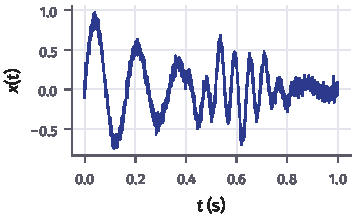
\includegraphics[height=2.2cm]{tipos_escalar_1d}\\[-1mm]{\footnotesize audio: $x(t)$}} &
      \parbox{4.6cm}{\centering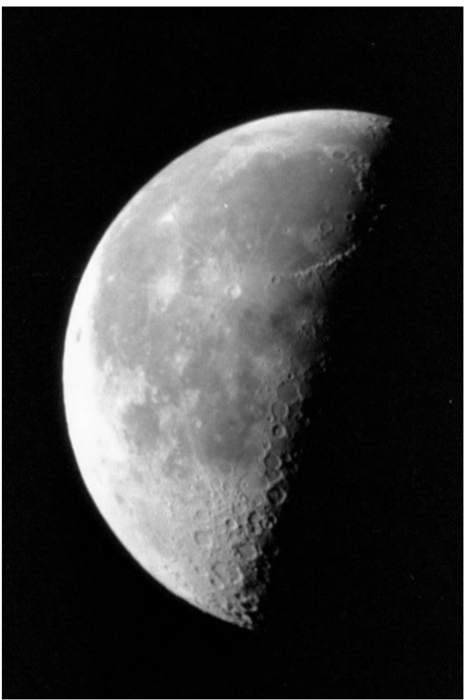
\includegraphics[height=2.2cm]{imagen_bn}\\[-0.5mm]{\footnotesize imagen en grises: $x(u,v)$}} \\[2mm]
    \rotatebox{90}{\textbf{\color{pdsrojo}Vectorial}} &
      \parbox{4.6cm}{\centering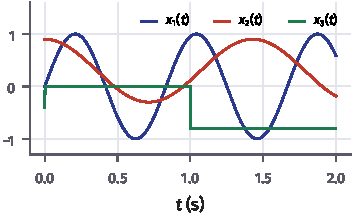
\includegraphics[height=2.2cm]{tipos_vectorial_1d}\\[-1mm]{\footnotesize acelerómetro: $[x_1(t)\ x_2(t)\ x_3(t)]$}} &
      \parbox{4.6cm}{\centering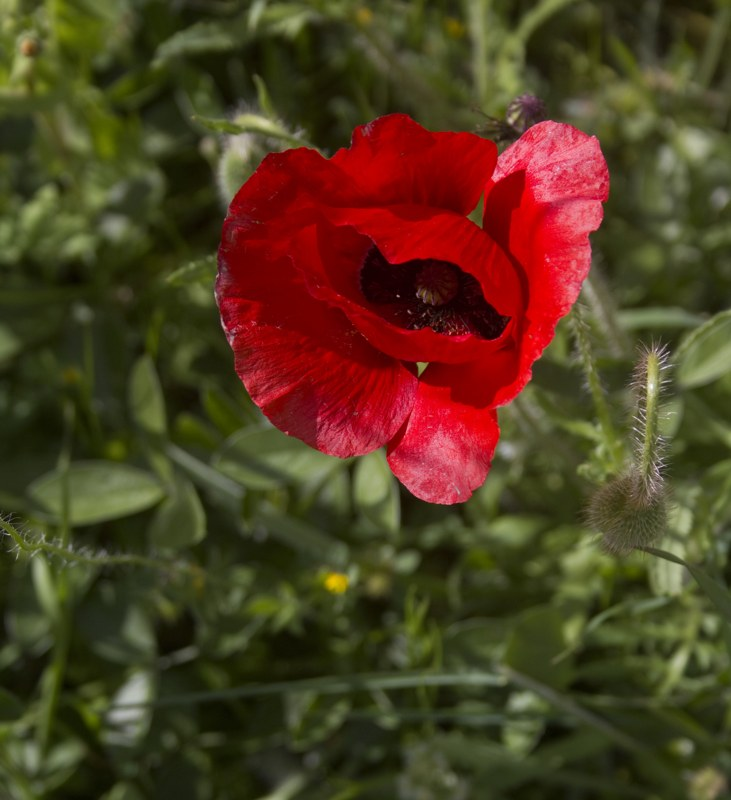
\includegraphics[height=2.2cm]{imagen_color}\\[-0.5mm]{\footnotesize imagen RGB: $[x_R\ x_G\ x_B](u,v)$}}
  \end{tabular}
\end{frame}

\begin{frame}{Variable independiente y amplitud}
  \begin{columns}[c]
    \begin{column}{0.45\textwidth}
      \small
      \begin{itemize}
        \item Variable independiente
        \begin{itemize}
          \item \alert{continua}: $x(t)$, $t\in\R$
          \item \alert{discreta}: $x[n]$, $n\in\Z$
        \end{itemize}
        \item Amplitud
        \begin{itemize}
          \item continua: $x\in\R$ (o $\C$)
          \item discreta: $x\in S$, conjunto finito o numerable, p.\,ej. $S=\set{k\Delta}$
        \end{itemize}
      \end{itemize}
      \smallskip
      {\footnotesize
      \begin{tabular}{@{}lll@{}}
        \toprule
        & ampl. cont. & ampl. disc.\\\midrule
        $t$ continuo & analógica & cuantificada\\
        $n$ discreto & muestreada & \alert{digital}\\\bottomrule
      \end{tabular}}
    \end{column}
    \begin{column}{0.53\textwidth}
      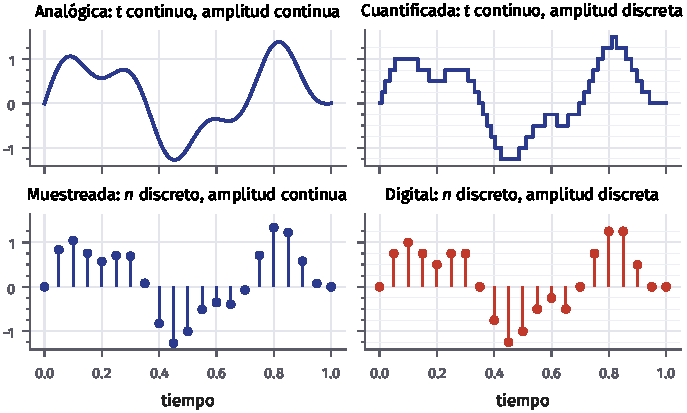
\includegraphics[width=0.84\linewidth]{analogica_digital}
    \end{column}
  \end{columns}
  \nota{Un computador solo representa señales digitales: discretas en tiempo y en amplitud.}
\end{frame}

\begin{frame}{Deterministas y aleatorias}
  \begin{itemize}
    \item \alert{Determinista}: su valor en cada instante está fijado por una expresión, una tabla o una regla. Se puede predecir.
    \item \alert{Aleatoria} o \alert{estocástica}: su valor en cada instante es una variable aleatoria; solo se describe estadísticamente (densidad de probabilidad, media, autocorrelación\ldots).
  \end{itemize}
  \begin{center}
    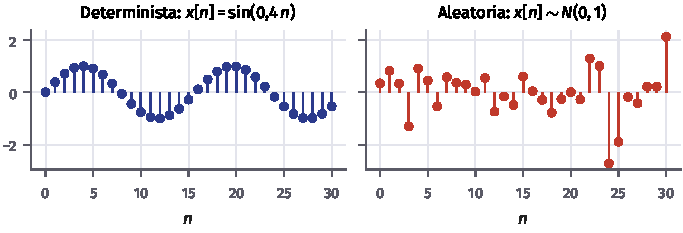
\includegraphics[width=0.66\linewidth]{determinista_aleatoria}
  \end{center}
  \nota{El ruido de un sensor, la voz o el tráfico de una red se modelan como señales aleatorias (Tema 6).}
\end{frame}

\begin{frame}{Periódicas y aperiódicas}
  \begin{definicion}[Señal periódica]
    \begin{tabular}{@{}ll@{}}
      Continua: & $x(t+T)=x(t)\quad\forall t$, \ con $T>0$\\
      Discreta: & $x[n+N]=x[n]\quad\forall n$, \ con $N\in\Z^+$
    \end{tabular}\\[1mm]
    El \alert{periodo fundamental} ($T_0$ o $N_0$) es el menor periodo positivo. Si $T$ es periodo, también lo es $lT$ para todo $l\in\Z$.
  \end{definicion}
  \begin{center}
    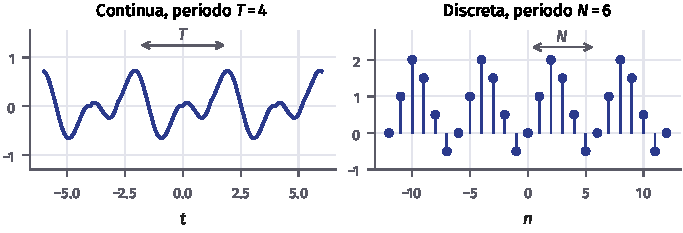
\includegraphics[width=0.52\linewidth]{periodicas}
  \end{center}
  \vspace{-3mm}
  {\small \alert{Aperiódica}: no cumple la relación para ningún periodo. La suma de dos periódicas solo es periódica si el cociente de periodos es racional: $\cos(2t)+\cos(3t)$ tiene $T_0=2\pi$; $\cos t+\cos(\pi t)$ no es periódica.}
\end{frame}

\begin{frame}{Pares e impares}
  \begin{columns}[c]
    \begin{column}{0.5\textwidth}
      \begin{itemize}
        \item \alert{Par} (simetría respecto al eje vertical)\\
          $x(t)=x(-t)$, \quad $x[n]=x[-n]$
        \item \alert{Impar} (simetría respecto al origen)\\
          $x(t)=-x(-t)$, \quad $x[n]=-x[-n]$\\
          \gris{\small En particular $x(0)=0$ y $x[0]=0$.}
      \end{itemize}
    \end{column}
    \begin{column}{0.48\textwidth}
      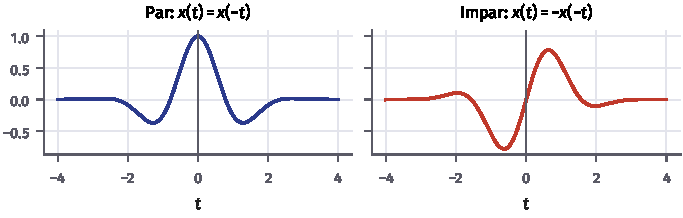
\includegraphics[width=\linewidth]{par_impar}
    \end{column}
  \end{columns}
  \bigskip
  \begin{block}{Descomposición par–impar}
    Toda señal se escribe de forma única como $x=x_p+x_i$, con
    \[
      x_p(t)=\frac{x(t)+x(-t)}{2},\qquad x_i(t)=\frac{x(t)-x(-t)}{2}
    \]
    \vspace{-2mm}
    {\small\gris{Igual en discreto. Propiedades: par·par y impar·impar son pares; par·impar es impar.}}
  \end{block}
\end{frame}

\begin{frame}{Descomposición par–impar: ejemplo}
  \[
    x[n]=2\,(0{,}8)^n u[n]\quad\Rightarrow\quad
    x_p[n]=\begin{cases}2 & n=0\\ (0{,}8)^{\abs{n}} & n\neq0\end{cases}\qquad
    x_i[n]=\sgn[n]\,(0{,}8)^{\abs{n}}
  \]
  \begin{center}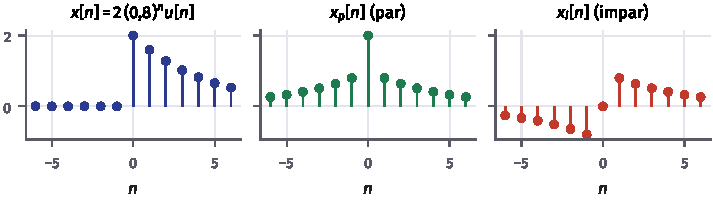
\includegraphics[width=0.85\linewidth]{descomposicion_par_impar}\end{center}
  \nota{Comprobación: $x_p[n]+x_i[n]$ vale $2(0{,}8)^n$ para $n\ge0$ y $0$ para $n<0$.}
\end{frame}

\begin{frame}{Causales, no causales y anticausales}
  \begin{center}
    \renewcommand{\arraystretch}{1.25}
    \begin{tabular}{@{}lll@{}}
      \toprule
      & Continua & Discreta\\\midrule
      \alert{Causal} & $x(t)=0\quad\forall t<0$ & $x[n]=0\quad\forall n<0$\\
      \alert{Anticausal} & $x(t)=0\quad\forall t>0$ & $x[n]=0\quad\forall n>0$\\
      \alert{No causal} & $x(t)\neq0$ para algún $t<0$ & $x[n]\neq0$ para algún $n<0$\\\bottomrule
    \end{tabular}
  \end{center}
  \begin{center}
    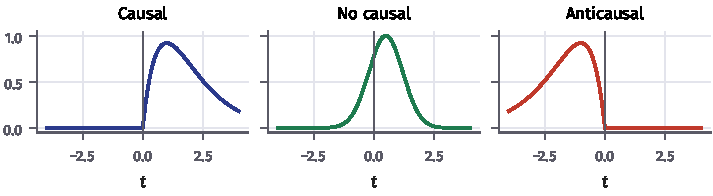
\includegraphics[width=0.7\linewidth]{causalidad}
  \end{center}
  \nota{El nombre viene de los sistemas: la respuesta al impulso de un sistema causal (físicamente realizable en tiempo real) es una señal causal.}
\end{frame}

\begin{frame}{Energía y potencia}
  \begin{center}
    \renewcommand{\arraystretch}{2.1}
    \begin{tabular}{@{}lll@{}}
      & Continua & Discreta\\
      \alert{Energía} & $\displaystyle E_x=\int_{-\infty}^{\infty}\abs{x(t)}^2\dd t$ & $\displaystyle E_x=\sum_{n=-\infty}^{\infty}\abs{x[n]}^2$\\
      \alert{Potencia media} & $\displaystyle P_x=\lim_{T\to\infty}\frac{1}{2T}\int_{-T}^{T}\abs{x(t)}^2\dd t$ & $\displaystyle P_x=\lim_{N\to\infty}\frac{1}{2N+1}\sum_{n=-N}^{N}\abs{x[n]}^2$
    \end{tabular}
  \end{center}
  \begin{itemize}\small
    \item \alert{Señal de energía}: $0<E_x<\infty$ (y entonces $P_x=0$). Típicamente limitadas en el tiempo o que decaen.
    \item \alert{Señal de potencia}: $0<P_x<\infty$ (y entonces $E_x=\infty$). Periódicas, escalón, ruido estacionario.
    \item Para una señal periódica basta un periodo: $P_x=\frac{1}{T_0}\int_{T_0}\abs{x(t)}^2\dd t$.
    \item Hay señales que no son de ninguno de los dos tipos, como la rampa.
  \end{itemize}
\end{frame}

\begin{frame}{Energía y potencia: tipos de señales}
  \begin{center}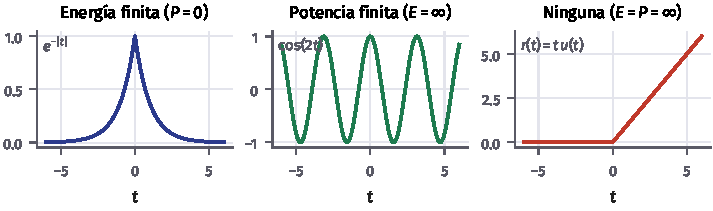
\includegraphics[width=0.9\linewidth]{energia_potencia}\end{center}
  \begin{itemize}\small
    \item Energía finita $\Rightarrow$ potencia nula: $P_x=\lim E_{[-T,T]}/2T=0$.
    \item Potencia finita no nula $\Rightarrow$ energía infinita.
    \item Las señales «físicas» observadas durante un tiempo finito siempre tienen energía finita; los modelos ideales (sinusoides eternas, escalón) son de potencia.
  \end{itemize}
\end{frame}

\begin{frame}{Energía y potencia: ejemplos}
  \begin{ejemplo}[Exponencial causal]
    $x[n]=a^n u[n]$ con $\abs{a}<1$: \quad
    $E_x=\displaystyle\sum_{n=0}^{\infty}\abs{a}^{2n}=\frac{1}{1-\abs{a}^2}$ \quad (señal de energía).
  \end{ejemplo}
  \begin{ejemplo}[Sinusoide]
    $x(t)=A\cos(\omega_0t+\phi)$: \quad $P_x=\dfrac{1}{T_0}\displaystyle\int_0^{T_0}A^2\cos^2(\omega_0t+\phi)\dd t=\dfrac{A^2}{2}$ \quad (señal de potencia).
  \end{ejemplo}
  \begin{ejemplo}[Escalón]
    $u(t)$: \quad $E=\infty$, \quad $P=\lim_{T\to\infty}\frac{1}{2T}\int_0^T1\dd t=\frac12$.
  \end{ejemplo}
\end{frame}

\begin{frame}{En código: energía y potencia}
  Aproximamos los límites con sumas finitas y comparamos con los valores teóricos de los ejemplos.
  \medskip
  \codigo{energia_potencia}
\end{frame}

\begin{frame}{Señales complejas}
  \begin{columns}[c]
    \begin{column}{0.52\textwidth}
      \small
      $x\in\C$ se describe con dos señales reales:
      \[
        x=\Re\{x\}+j\Im\{x\}=\abs{x}\,\e^{j\arg x}
      \]
      \vspace{-4mm}
      \begin{align*}
        \Re\{x\}&=\abs{x}\cos(\arg x)\\
        \Im\{x\}&=\abs{x}\sin(\arg x)\\
        \abs{x}&=\sqrt{\Re\{x\}^2+\Im\{x\}^2}\\
        \arg x&=\atantwo\big(\Im\{x\},\Re\{x\}\big)
      \end{align*}
      {\small\gris{$\arctan(\Im/\Re)$ solo da el ángulo correcto si $\Re\{x\}>0$: hay que tener en cuenta el cuadrante (\texttt{np.angle}, \texttt{angle}).}}
    \end{column}
    \begin{column}{0.46\textwidth}
      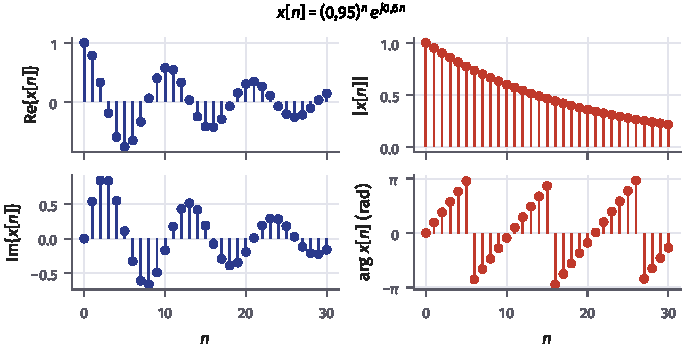
\includegraphics[width=\linewidth]{compleja}
    \end{column}
  \end{columns}
  \nota{Aparecen en las series y transformadas de Fourier y, en comunicaciones, para representar a la vez amplitud y fase (señal en banda base I/Q).}
\end{frame}

\begin{frame}{Simetrías de las señales complejas}
  Con $x=a+jb$ ($a,b$ reales) y $^*$ el conjugado:
  \begin{center}
    \renewcommand{\arraystretch}{1.3}
    \begin{tabular}{@{}lll@{}}
      \toprule
      Señal & Condición & Consecuencia\\\midrule
      \alert{Real} & $x(t)=x^*(t)$ & $b(t)=0$\\
      \alert{Imaginaria pura} & $x(t)=-x^*(t)$ & $a(t)=0$\\
      \alert{Hermítica} (conjugada simétrica) & $x(t)=x^*(-t)$ & $a$ par, $b$ impar\\
      \alert{Antihermítica} & $x(t)=-x^*(-t)$ & $a$ impar, $b$ par\\\bottomrule
    \end{tabular}
  \end{center}
  \begin{block}{Por qué importa}
    La transformada de Fourier de una señal \alert{real} es \alert{hermítica}: $X(-j\omega)=X^*(j\omega)$. Por eso su módulo es par y su fase impar, y basta representar las frecuencias positivas.
  \end{block}
\end{frame}

% =====================================================================
\section{Señales básicas}

\begin{frame}{Impulso continuo: delta de Dirac}
  \begin{columns}[c]
    \begin{column}{0.56\textwidth}
      \small
      \begin{itemize}
        \item Límite de pulsos de área unidad:\\ $\delta(t)=\lim_{\varepsilon\to0}\frac{1}{\varepsilon}\rect(t/\varepsilon)$.
        \item No es una función ordinaria: se define por su efecto en una integral (es una distribución).
      \end{itemize}
      \begin{block}{Propiedades}
        \small
        \begin{itemize}
          \item Selección: $\displaystyle\int_{-\infty}^{\infty}x(t)\,\delta(t-t_0)\dd t=x(t_0)$
          \item $x(t)\,\delta(t-t_0)=x(t_0)\,\delta(t-t_0)$
          \item Escalado: $\delta(at)=\dfrac{1}{\abs{a}}\delta(t)$, \ $a\neq0$
          \item Elemento neutro: $(x\conv\delta)(t)=x(t)$
        \end{itemize}
      \end{block}
    \end{column}
    \begin{column}{0.42\textwidth}
      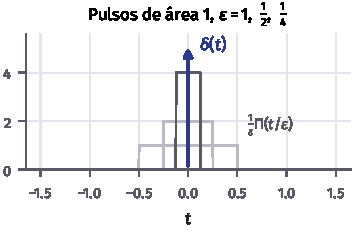
\includegraphics[width=\linewidth]{impulso_dirac}
    \end{column}
  \end{columns}
\end{frame}

\begin{frame}{Impulso discreto: delta de Kronecker}
  \begin{columns}[c]
    \begin{column}{0.56\textwidth}
      \[
        \delta[n]=\begin{cases}1 & n=0\\0 & n\neq0\end{cases}
      \]
      \begin{itemize}
        \item Es una secuencia ordinaria: no hay problemas de definición.
        \item Toda secuencia es una suma de impulsos desplazados y ponderados:
        \[x[n]=\sum_{k=-\infty}^{\infty}x[k]\,\delta[n-k]\]
        \item Elemento neutro de la convolución: $(x\conv\delta)[n]=x[n]$.
      \end{itemize}
    \end{column}
    \begin{column}{0.4\textwidth}
      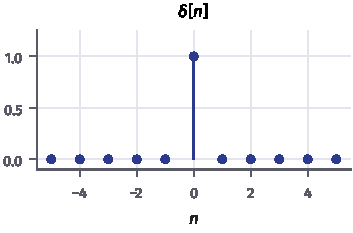
\includegraphics[width=\linewidth]{impulso_kronecker}
    \end{column}
  \end{columns}
  \nota{La descomposición en impulsos es la base para obtener la respuesta de un sistema LTI (Parte 3).}
\end{frame}

\begin{frame}{Escalón y rampa}
  \begin{columns}[c]
    \begin{column}{0.52\textwidth}
      \small
      \alert{Escalón unitario}
      \[
        u(t)=\begin{cases}1 & t>0\\0 & t<0\end{cases}\qquad
        u[n]=\begin{cases}1 & n\ge0\\0 & n<0\end{cases}
      \]
      $u(t)=\int_{-\infty}^{t}\delta(\tau)\dd\tau$, \ $\delta(t)=\dv{u(t)}{t}$\\[1mm]
      $u[n]=\sum_{k=-\infty}^{n}\delta[k]$, \ $\delta[n]=u[n]-u[n-1]$\\[1mm]
      \gris{El valor de $u(0)$ no afecta a ninguna integral; se suele tomar $u(0)=1$ o $\tfrac12$.}
      \medskip

      \alert{Rampa}: \ $r(t)=t\,u(t)$, \quad $r[n]=n\,u[n]$\\[1mm]
      $r(t)=\int_{-\infty}^{t}u(\tau)\dd\tau$, \ $u(t)=\dv{r(t)}{t}$\\[1mm]
      $r[n]=\sum_{k=-\infty}^{n-1}u[k]$, \ $u[n]=r[n+1]-r[n]$
    \end{column}
    \begin{column}{0.46\textwidth}
      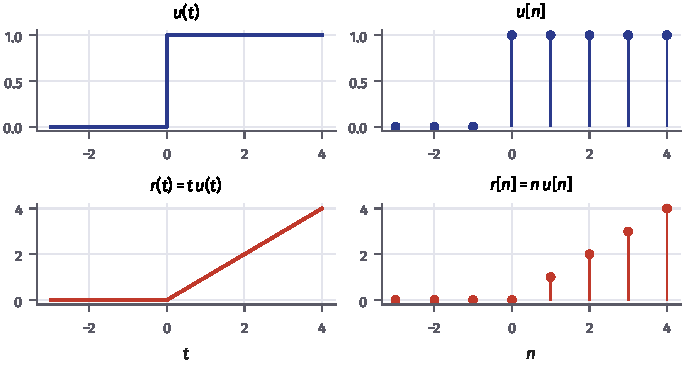
\includegraphics[width=\linewidth]{escalon_rampa}
      \nota{Multiplicar por $u(t)$ o $u[n]$ hace causal cualquier señal.}
    \end{column}
  \end{columns}
\end{frame}

\begin{frame}{Pulsos rectangular y triangular}
  \begin{columns}[c]
    \begin{column}{0.5\textwidth}
      \[
        \rect(t)=\begin{cases}1 & \abs{t}\le\frac12\\[1mm]0 & \abs{t}>\frac12\end{cases}
      \]
      \[
        \tri(t)=\begin{cases}1-\abs{t} & \abs{t}\le1\\[1mm]0 & \abs{t}>1\end{cases}
      \]
      \begin{itemize}\small
        \item $\rect(t/T)$: pulso de anchura $T$ centrado en 0.
        \item $\tri(t)=(\rect\conv\rect)(t)$: el triangular es la convolución de dos rectangulares.
        \item Versión discreta: $p_L[n]=u[n]-u[n-L]$, pulso causal de $L$ muestras.
      \end{itemize}
    \end{column}
    \begin{column}{0.48\textwidth}
      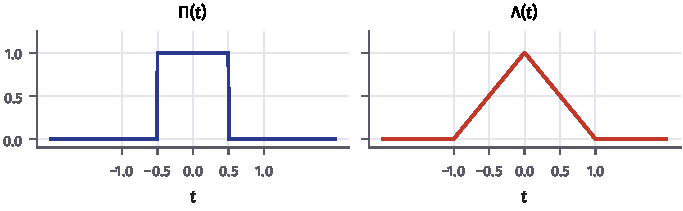
\includegraphics[width=\linewidth]{pulsos}
    \end{column}
  \end{columns}
\end{frame}

\begin{frame}{Exponencial compleja continua}
  \begin{columns}[c]
    \begin{column}{0.52\textwidth}
      \[x(t)=A\,\e^{j\omega_0 t}\]
      \begin{itemize}\small
        \item Periódica para todo $\omega_0\neq0$, con $T_0=\dfrac{2\pi}{\abs{\omega_0}}$:\\
          \gris{$\e^{j\omega_0(t+T_0)}=\e^{j\omega_0t}\e^{j2\pi}=\e^{j\omega_0t}$}
        \item $\omega_0=2\pi f_0$: rad/s y Hz.
        \item Frecuencias distintas dan señales distintas, y cuanto mayor es $\abs{\omega_0}$ más rápido oscila.
      \end{itemize}
    \end{column}
    \begin{column}{0.46\textwidth}
      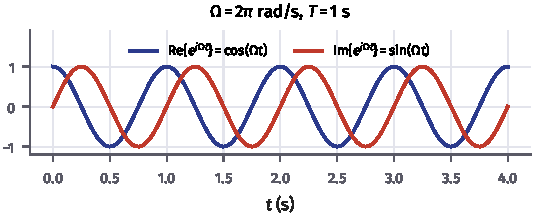
\includegraphics[width=\linewidth]{exp_compleja_continua}
    \end{column}
  \end{columns}
  \begin{block}{Fórmula de Euler}
    \[
      \e^{j\theta}=\cos\theta+j\sin\theta\quad\Rightarrow\quad
      \cos\theta=\frac{\e^{j\theta}+\e^{-j\theta}}{2},\qquad
      \sin\theta=\frac{\e^{j\theta}-\e^{-j\theta}}{2j}
    \]
  \end{block}
\end{frame}

\begin{frame}{Exponencial continua general}
  \[
    x(t)=C\,\e^{at},\quad C,a\in\C
    \qquad\left.\begin{array}{l}C=\abs{C}\e^{j\phi}\\ a=r+j\omega_0\end{array}\right\}
    \;\Rightarrow\; x(t)=\abs{C}\,\e^{rt}\,\e^{j(\omega_0t+\phi)}
  \]
  \begin{itemize}
    \item Sinusoide compleja con envolvente exponencial: decreciente ($r<0$), constante ($r=0$) o creciente ($r>0$).
    \item Si $a$ es real ($\omega_0=0$) es la exponencial real $C\e^{rt}$.
    \item Son las respuestas naturales de los sistemas descritos por ecuaciones diferenciales lineales: $a$ es un \alert{polo}.
  \end{itemize}
  \begin{center}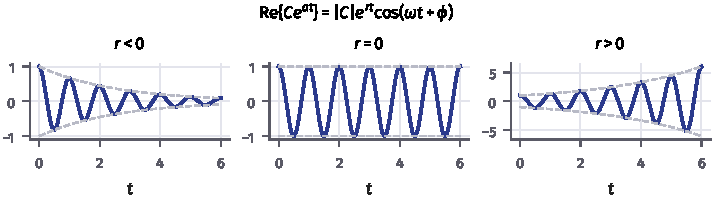
\includegraphics[width=0.62\linewidth]{exp_general_continua}\end{center}
\end{frame}

\begin{frame}{Exponencial compleja discreta: periodicidad}
  \[x[n]=A\,\e^{j\Omega_0 n},\qquad \Omega_0=2\pi F_0\ \text{(rad/muestra)}\]
  \begin{importante}[No siempre es periódica]
    $x[n+N]=x[n]\iff \e^{j\Omega_0N}=1\iff \Omega_0N=2\pi k$, es decir, $F_0=\dfrac{\Omega_0}{2\pi}=\dfrac{k}{N}$ debe ser \alert{racional}.\\[1mm]
    Con $k/N$ irreducible, el periodo fundamental es $N$.
  \end{importante}
  \vspace{-1mm}
  \begin{ejemplo}
    \begin{itemize}\small
      \item $\cos(\pi n/4)$: $F_0=1/8$, periodo $N=8$.
      \item $\cos(3\pi n/8)$: $F_0=3/16$, periodo $N=16$ (¡no $16/3$!).
      \item $\cos(0{,}4\,n)$: $F_0=0{,}2/\pi$ es irracional, \alert{no es periódica} aunque $\cos(0{,}4\,t)$ sí lo sea.
    \end{itemize}
  \end{ejemplo}
\end{frame}

\begin{frame}{Exponencial compleja discreta: frecuencias equivalentes}
  \begin{importante}[Frecuencias que difieren en $2\pi$ dan la misma secuencia]
    \[\e^{j(\Omega_0+2\pi k)n}=\e^{j\Omega_0n}\,\e^{j2\pi kn}=\e^{j\Omega_0n}\qquad\forall k\in\Z\]
    Basta un intervalo de longitud $2\pi$: $0\le\Omega<2\pi$ o $-\pi\le\Omega<\pi$.
  \end{importante}
  \begin{itemize}\small
    \item La oscilación más rápida posible está en $\Omega=\pi$: $\e^{j\pi n}=(-1)^n$.
    \item Las frecuencias bajas están cerca de $\Omega=0$ \emph{y} cerca de $\Omega=2\pi$.
    \item Origen del \alert{aliasing} al muestrear (Tema 2).
  \end{itemize}
  \begin{center}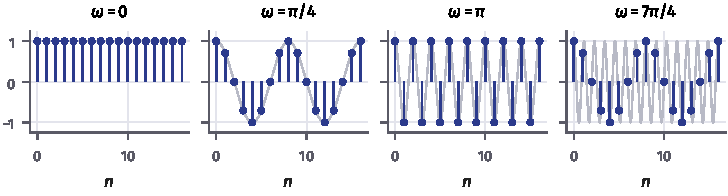
\includegraphics[width=0.75\linewidth]{coseno_discreto_frecuencias}\end{center}
  \vspace{-2mm}
  \herramienta{html/T1\_Exponencial Continua vs. Discreta.html}
\end{frame}

\begin{frame}{Exponencial discreta general}
  \[
    x[n]=C\,\alpha^n,\quad C,\alpha\in\C
    \qquad\left.\begin{array}{l}C=\abs{C}\e^{j\phi}\\ \alpha=\abs{\alpha}\e^{j\Omega_0}\end{array}\right\}
    \;\Rightarrow\; x[n]=\abs{C}\,\abs{\alpha}^n\,\e^{j(\Omega_0n+\phi)}
  \]
  \begin{itemize}
    \item Envolvente decreciente ($\abs{\alpha}<1$), constante ($\abs{\alpha}=1$) o creciente ($\abs{\alpha}>1$).
    \item Si $\alpha$ es real y negativo, la señal alterna de signo.
    \item Son las respuestas naturales de las ecuaciones en diferencias: $\alpha$ es un polo en el plano $z$.
  \end{itemize}
  \begin{center}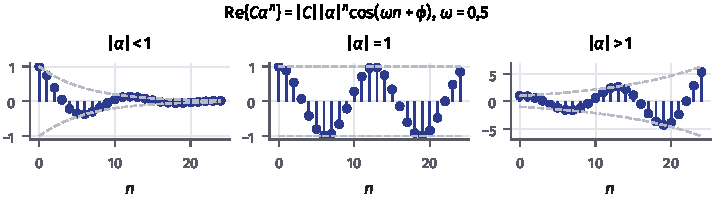
\includegraphics[width=0.62\linewidth]{exp_general_discreta}\end{center}
\end{frame}

\begin{frame}{Sa, sinc y signo}
  \begin{columns}[c]
    \begin{column}{0.48\textwidth}
      \[
        \Sa(t)=\frac{\sin t}{t},\qquad
        \sinc(t)=\frac{\sin(\pi t)}{\pi t},
      \]
      con $\Sa(0)=\sinc(0)=1$. Así, $\sinc(t)=\Sa(\pi t)$.
      \begin{itemize}\small
        \item $\sinc$ se anula en los enteros no nulos.
        \item Es la transformada de Fourier del pulso rectangular y el interpolador ideal del Tema 2.
        \item \texttt{np.sinc} y \texttt{sinc} de Matlab calculan $\sin(\pi t)/(\pi t)$.
      \end{itemize}
      \[
        \sgn(t)=\begin{cases}1 & t>0\\0 & t=0\\-1 & t<0\end{cases}
      \]
    \end{column}
    \begin{column}{0.5\textwidth}
      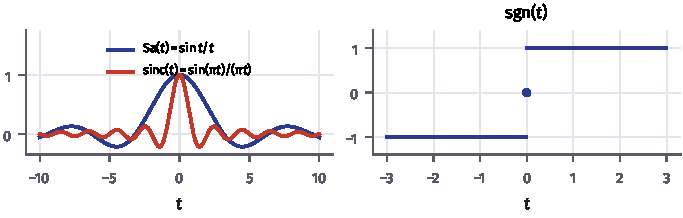
\includegraphics[width=\linewidth]{sa_sinc_signo}
    \end{column}
  \end{columns}
\end{frame}

\begin{frame}{Ondas periódicas y chirp}
  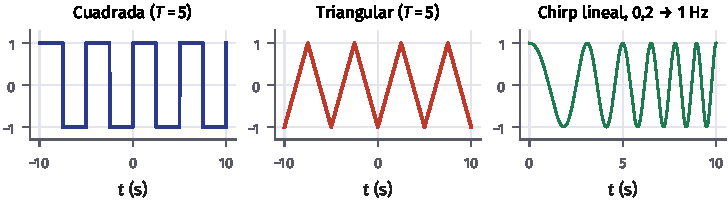
\includegraphics[width=\linewidth]{ondas}
  \begin{itemize}\small
    \item \alert{Cuadrada} y \alert{triangular}: periódicas, con armónicos impares (Parte 2).
    \item \alert{Chirp lineal}: $x(t)=\cos\!\big(2\pi(f_0t+\tfrac{\beta}{2}t^2)\big)$. Su frecuencia instantánea, $\frac{1}{2\pi}\dv{\theta}{t}=f_0+\beta t$, crece linealmente. Se usa en radar, sonar y para medir respuestas en frecuencia.
  \end{itemize}
\end{frame}

\begin{frame}{En código: señales básicas}
  \codigo{senales_basicas}
  \nota{Los ejemplos están en \texttt{teoría/T1/codigo/} y se ejecutan automáticamente para comprobar que funcionan.}
\end{frame}

\begin{frame}{En código: frecuencias discretas equivalentes}
  Las tres secuencias son la misma, aunque las frecuencias sean distintas:
  \medskip
  \codigo{alias_discreto}
\end{frame}

% =====================================================================
\section*{Resumen}
\begin{frame}{Conceptos importantes}
  \begin{columns}[T]
    \begin{column}{0.5\textwidth}
      \begin{itemize}
        \item Señal y sistema; notación $x(t)$ frente a $x[n]$.
        \item Clasificación de señales:
        \begin{itemize}\small
          \item analógica, muestreada, digital
          \item determinista o aleatoria
          \item periódica (periodo fundamental)
          \item par, impar, causal
          \item de energía o de potencia
          \item real, compleja, hermítica
        \end{itemize}
      \end{itemize}
    \end{column}
    \begin{column}{0.5\textwidth}
      \begin{itemize}
        \item Señales básicas: $\delta$, $u$, $r$, $\rect$, $\tri$, $\sinc$, $\sgn$, exponenciales.
        \item \alert{Diferencias entre la exponencial continua y la discreta}:
        \begin{itemize}\small
          \item $\e^{j\Omega_0n}$ solo es periódica si $\Omega_0/2\pi$ es racional.
          \item $\Omega_0$ y $\Omega_0+2\pi$ dan la misma secuencia.
        \end{itemize}
      \end{itemize}
    \end{column}
  \end{columns}
  \bigskip
  \gris{Apuntes del Tema 1, secciones 1–3 · Hoja de ejercicios, ejercicios 1–4 y 9.}
\end{frame}

\end{document}
